\begin{frame}{Заключение}

\begin{footnotesize}

Работа над этой презентацией не окончена. Актуальная версия расположена по~адресу
\url{http://mech.math.msu.su/~shvetz/54/inf/metapost/mpshort.pdf}.

При создании настоящего руководства использовались следующие технологии:
\hologo{LuaLaTeX}, \hologo{METAPOST}.

\bigskip


\begin{columns}%[onlytextwidth]
\column{.125\textwidth}
\centerline{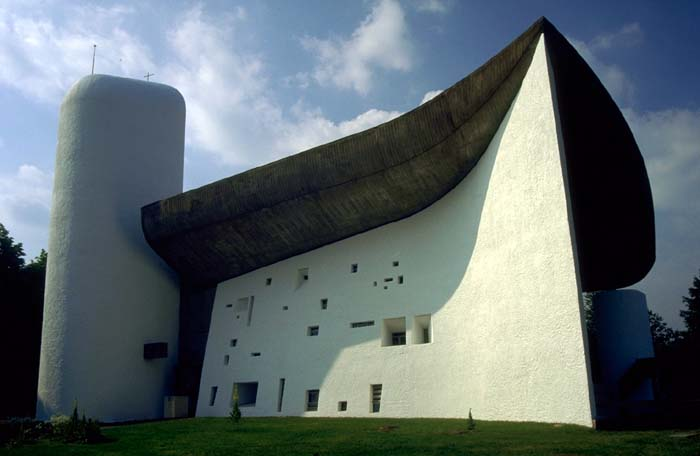
\includegraphics[width=.8\textwidth]{figure-ronchamp}}
\column{.825\textwidth}
Иллюстрация с~изображением капеллы в~Роншане архитектора Ле~Корбюзье
(Le~Corbusier) взята по~адресу
\url{http://home.broadpark.no/~lhellemo/gallery/architecture/Le_Corbusier_front.jpg}

\end{columns}

\medskip

\begin{columns}[onlytextwidth]
\column{.125\textwidth}
\centerline{\scalebox{.25}{\leavevmode
\begin{mplibcode}
beginfig(0)

numeric w, circ[], h, u;
u:=3bp;

w:=1200/36u;
circ0=.4u;
circ1=1.2u;
h:=w;

color gridcolor, integralcolor, moebiuscolor;
gridcolor=(.125, .25, .35);
moebiuscolor=1.5gridcolor;
integralcolor=1.5gridcolor;

wh[0]:=w; wh[1]:=h;
for i=0 upto 1:
  k[i]:=wh[i]/35; p[i]:=floor(4k[i]);
  s[i]:=floor(p[i]/2.5);
  q[i]:=wh[i]-7p[i]-2s[i]; r[i]:=round(q[i]/8); wh[i]:=2s[i]+7p[i]+8r[i];
endfor
w:=wh0; h:=wh1;
%TZh:=h/aspect_ratio;

path P;
%TZ currentpicture:=unitpixel xscaled wh0 yscaled wh1;
%TZ currentpicture:=unitsquare xscaled wh0 yscaled wh1;
%TZ P:=unitpixel xscaled (7p0+8r0) yscaled (7p1+8r1) shifted (s0,s1);
P:=unitsquare xscaled (7p0+8r0) yscaled (7p1+8r1) shifted (s0,s1);
%TZ addto currentpicture also -P;
fill P withcolor gridcolor;

P:=unitsquare xscaled p0 yscaled p1;
for m=0 upto 6:
	for n=0 upto 6:
		fill (P shifted ((s0+r0,s1+r1)+(m*(p0+r0),n*(p1+r1))))
			withcolor background;
	endfor
endfor

%%   Möbius band coordinates

z1=(0.11881w, .24587h);  z2=(.29938w, .59362h);  z3=(.56688w, .88119h);
z4=(0.72069w, .85444h);  z5=(.45319w, .56688h);  z6=(.28600w, .27931h);
z7=(0.12550w, .21912h);  z8=(.28600w, .24587h);  z9=(.58025w, .33281h);
z10=(0.88788w, .46656h); z11=(.83438w, .29938h); z12=(.54681w, .17900h);
z13=(0.21912w, .09206h); z14=(.76081w, .42644h); z15=(.64044w, .74075h);
z16=(0.74075w, .83438h); z17=(.88119w, .49331h); z18=(.82769w, .67388h);
z19=(0.70731w, .59362h); z20=(.60031w, .74744h); z21=(.76750w, .39969h);

%%   Integeral sign coordinates

wide:=.1w; bold:=.07w; vair:=.05h; bulb:=.07h;
penpos31(bulb,-90); penpos37(bulb,-90);
penpos32(vair,-90); penpos36(vair,-90);
penpos33(bold,0); penpos35(bold,0);
penpos34(wide,0);
z34=(.5w,.5h); z32=(.5w,1.03h);
z33+z35=z32+z36=z31+z37=(w,h);
y33=.8h; x33l=x34l-0.03w;
x31=.55w; y31l=y32l;

path S;
S=z34l..tension 4..z35l...z36l...z37l...z37r...z36r..tension 1.1..z35r...z34r..
  tension 4..z33r...z32r...z31r...z31l...z32l..tension 1.1..z33l...cycle;

fill z1--z6--z8--z7--cycle withcolor background;
fill z4--z16--z15--z20--cycle withcolor background;
fill z10--z17--z14--z21--cycle withcolor background;
%erase fill flex(z1,z2,z3) & z3--z4 & flex(z4,z5,z6) & z6--z1 & cycle;
pickup pencircle scaled circ0;
fill flex(z1,z2,z3) & z3--z4 & flex(z4,z5,z6) & z6--z1 & cycle
		withcolor moebiuscolor;
draw flex(z1,z2,z3) & z3--z4 & flex(z4,z5,z6) & z6--z1 & cycle
		withcolor black;
%erase fill flex(z14,z19,z15) & z15--z16 & flex(z16,z18,z17) & z17--z14 & cycle;
fill flex(z14,z19,z15) & z15--z16 & flex(z16,z18,z17) & z17--z14 & cycle
		withcolor moebiuscolor;
draw flex(z14,z19,z15) & z15--z16 & flex(z16,z18,z17) & z17--z14 & cycle
		withcolor black;
pickup pencircle scaled circ1;
fill S withcolor integralcolor;
draw S withcolor black;
pickup pencircle scaled circ0;
filldraw S withcolor integralcolor;
%erase fill flex(z7,z9,z10) & z10--z11 & flex(z11,z12,z13) & z13--z7 & cycle;
fill flex(z7,z9,z10) & z10--z11 & flex(z11,z12,z13) & z13--z7 & cycle
		withcolor moebiuscolor;
%pickup pencircle scaled circ1;
draw flex(z7,z9,z10) & z10--z11 & flex(z11,z12,z13) & z13--z7 & cycle
		withcolor black;

endfig
\end{mplibcode}
}}
\column{.825\textwidth}
Изображение логотипа механико"=математического факультета МГУ
имени М.~В.~Ломоносова первоначально было подготовлено С.~В.~Голованем
в~системе~\hologo{METAFONT} и~адаптировано автором для \hologo{METAPOST}.

\end{columns}

\medskip

\begin{columns}
\column{.125\textwidth}
\centerline{
\includegraphics[width=.8\textwidth]{aiga_hotel_information1}}
\column{.825\textwidth}
Пиктограммы взяты с~сайта \url{http://aiga.org}.

\end{columns}

\medskip

\begin{columns}
\column{.125\textwidth}
\centerline{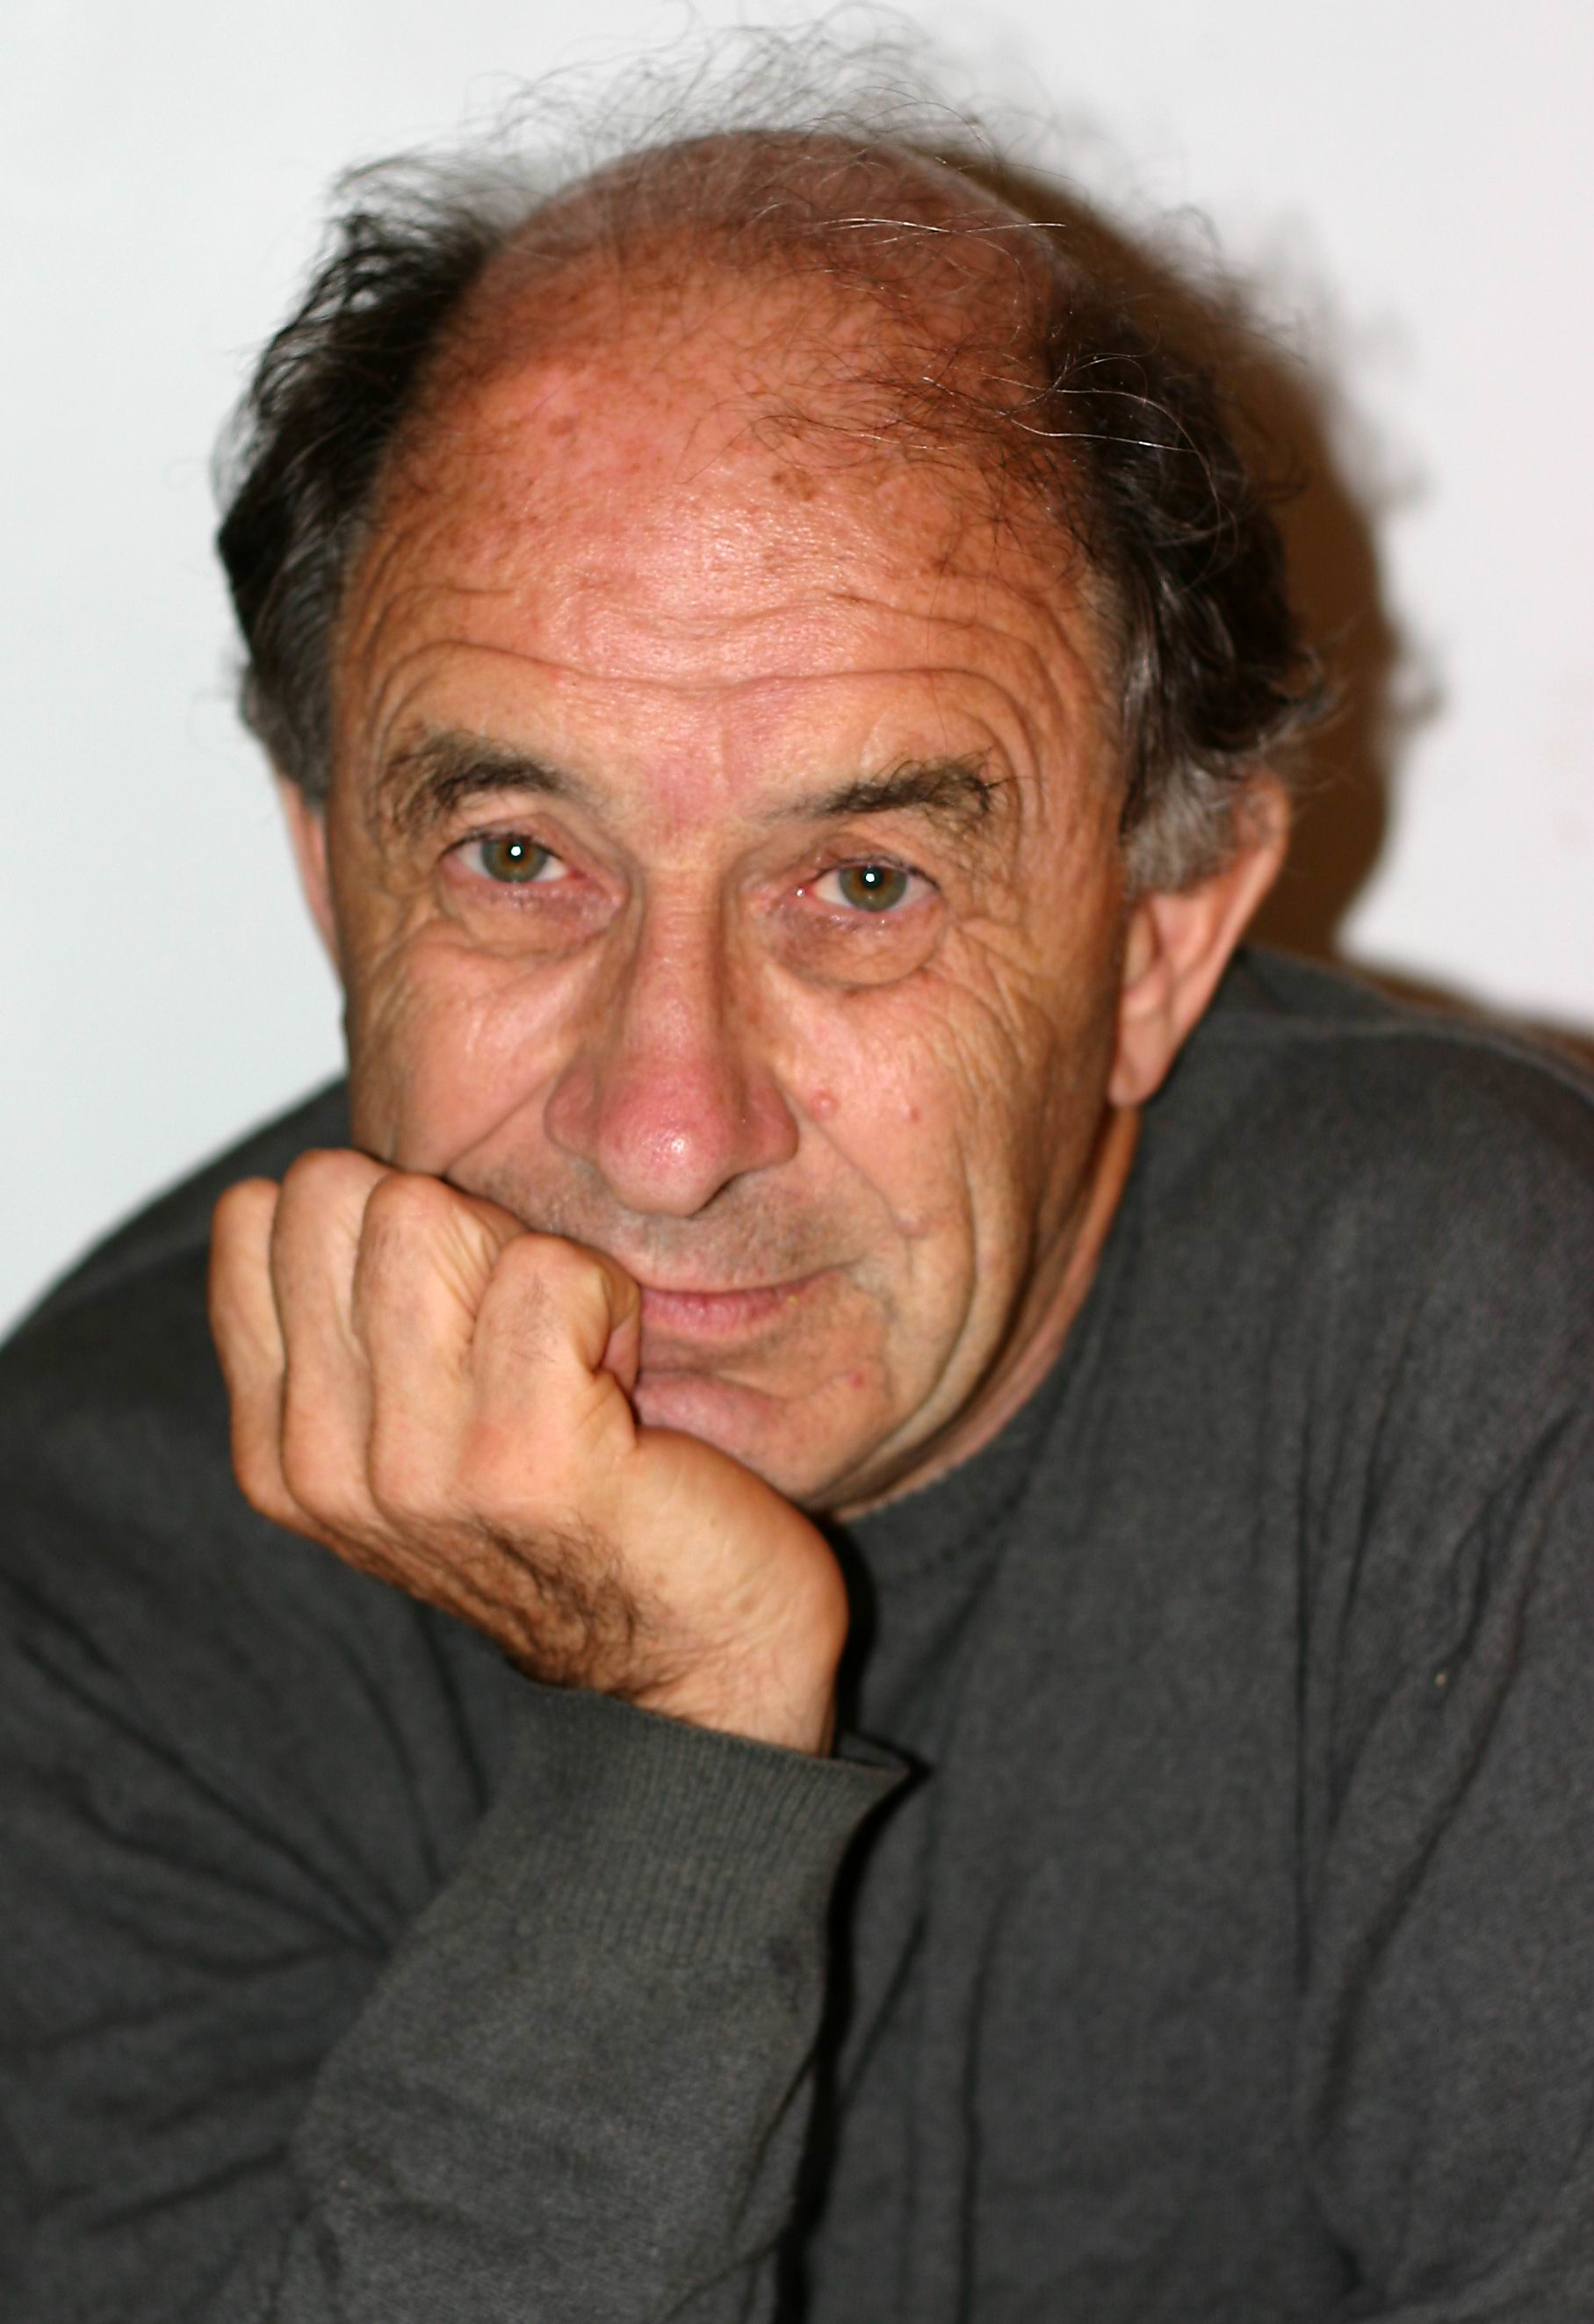
\includegraphics[width=.5\textwidth]{figure-arnold}}
\column{.825\textwidth}
Фотография В.~И.~Арнольда взята на Википедии:
\url{https://commons.wikimedia.org/wiki/File:Vladimir_Arnold-1.jpg}.

\end{columns}

\end{footnotesize}
\end{frame}
